% Questo è il mio primo documento serio scritto in Latex, quindi potrebbe contenere degli orrori
% Chiedo umilmente scusa xD
\documentclass[a4paper, titlepage, oneside]{scrbook}
\usepackage[italian]{babel}
\usepackage[utf8]{inputenc}
\usepackage[hidelinks]{hyperref}
\usepackage{amsmath}
\usepackage{amssymb}
\usepackage{mathtools}
\usepackage{tikz}
\usetikzlibrary{arrows,calc,patterns,angles,quotes}
\usepackage{pgfplots}
\usepgfplotslibrary{fillbetween}

%opening
\title{Appunti di Elaborazione di Segnali e Immagini}
\author{Matteo Iervasi}
\date{ }

\begin{document}

\maketitle

\newpage
	\tableofcontents
\newpage

\chapter{Introduzione}
\section{Che cos'è un segnale?}
Si definisce \textbf{segnale} una qualsiasi grandezza fisica che varia nel tempo e trasporta informazione. 
In generale esistono diversi tipi di segnali, ma in natura sono quasi sempre casuali e continui.

Una prima grossa suddivisione della teoria dei segnali si basa sul tipo di segnale: i segnali \textbf{deterministici}, 
di cui è possibile predire il valore in un qualunque istante a piacere, e i segnali \textbf{stocastici} o \textbf{aleatori}, 
il cui valore non è prevedibile, ma su cui è possibile ottenere soltanto delle proprietà statistiche.
Altra suddivisione è quella in segnali \textbf{continui} e \textbf{discreti}, ai quali si associano rispettivamente le comunicazioni \textit{analogiche} e le comunicazioni \textit{digitali}.

Parte della teoria dei segnali è profondamente connessa con la \textbf{teoria dei sistemi}, in quanto molti segnali transitano come input 
in sistemi che elaborano ovvero trasformano il segnale in ingresso restituendo in uscita un certo output.

\section{Che cos'è un sistema?}
Possiamo definire un \textbf{sistema} (dinamico) come un modello matematico che rappresenta un oggetto che evolve nel tempo.
\begin{figure}[h]
	\centering
	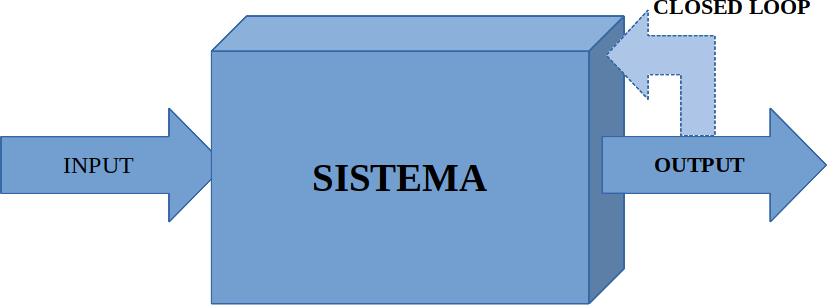
\includegraphics[width=0.7\linewidth]{img/sistema}
	\caption[Schema di un sistema]{Schema di un sistema}
	\label{fig:sistema}
\end{figure}

\section{Classificazione dei segnali}
Come accennato prima, possiamo suddividere i segnali in diverse categorie:
\begin{itemize}
	\item Continui nel tempo - Discreti nel tempo
	\item Analogici - Digitali
	\item Periodici - Aperiodici
	\item Causali e non causali
	\item Pari e dispari
	\item Deterministici - Casuali
	\item Segnali di energia - Segnali di potenza
	\item ...
\end{itemize}
È importante notare come le suddivisioni sopra elencate non siano esclusive tra loro, ci sono ad esempio segnali di potenza periodici, analogici e casuali, ecc.

\subsection{Segnali a tempo continuo e a tempo discreto}
Un segnale si definisce \textbf{a tempo continuo} quando il suo dominio ha la stessa cardinalità dei numeri reali, ed è quindi specificato per ogni reale.
Viceversa si definisce \textbf{discreto} quando il suo dominio ha la stessa cardinalità dei numeri naturali, ed è quindi specificato per valori discreti.

\begin{figure}[h]
	\centering
	\begin{tikzpicture}
	\begin{axis}[
		axis lines=left,
		xlabel=Tempo,
		ylabel=Ampiezza,
		trig format plots=rad,
	]
	\addplot[
		domain=0:4*pi,
		samples=360,
		color=blue,
		line width=1.25pt,
	]{sin(x)};
	\addlegendentry{Tempo continuo}
	\addplot[
		domain=0:4*pi,
		samples=360,
		color=red,
		line width=1.25pt,
		loosely dotted,
		line cap=round,
	]{sin(x+1)};
	\addlegendentry{Tempo discreto}
	\end{axis}
\end{tikzpicture}
\caption{Due segnali sinusoidali, uno continuo e l'altro discreto}
\label{fig:sinusoidi_tempo_continuo_discreto}
\end{figure}

\subsection{Segnali analogici e digitali}
Se parlando del dominio abbiamo i segnali a tempo continuo e a tempo discreto, possiamo distinguere i segnali analogici e digitali guardando i valori assunti dal codominio.
Quando l'ampiezza di un segnale può assumere qualsiasi valore in un intervallo continuo, parliamo di segnale \textbf{analogico}, viceversa quando assume solo un insieme
finito di valori parliamo di segnale \textbf{digitale}. In quest'ultimo caso il segnale si dice "\textit{quantizzato}".

\begin{figure}[h]
	\centering
	\begin{tikzpicture}
	\begin{axis}[
		scale only axis,
		height=5cm,
		width=9cm,
		axis lines=left,
		xlabel=Tempo,
		ylabel=Ampiezza,
		trig format plots=rad,
	]
	\addplot[
		domain=0:8*pi,
		samples=360,
		color=blue,
		line width=1.25pt,
	]{sin(x)};
	\addlegendentry{Segnale analogico}
	\addplot+[
		color=red,
		mark=none,
		const plot,
		line width=1.25pt,
	]
	coordinates {
		(0,0.00)
		(1,0.84)
		(2,0.91)
		(3,0.14)
		(4,-0.76)
		(5,-0.96)
		(6,-0.28)
		(7,0.66)
		(8,0.99)
		(9,0.41)
		(10,-0.54)
		(11,-1.00)
		(12,-0.54)
		(13,0.42)
		(14,0.99)
		(15,0.65)
		(16,-0.29)
		(17,-0.96)
		(18,-0.75)
		(19,0.15)
		(20,0.91)
		(21,0.84)
		(22,-0.01)
		(23,-0.85)
		(24,-0.91)
	};
	\addlegendentry{Segnale digitale}
	\end{axis}
\end{tikzpicture}
\caption{Confronto fra segnale analogico e digitale}
\label{fig:analogico_vs_digitale}
\end{figure}

\subsection{Segnali periodici e aperiodici}
Un segnale è \textbf{periodico} se esiste una costante positiva $T_{0}$ tale che
$$
	f(t+T_{0})=f(t) \qquad \forall t
$$
Il più piccolo valore di $T_{0}$ che soddisfa questa relazione è chiamato \textbf{periodo} della funzione. Un segnale periodico rimane invariato quando viene spostato
nel tempo. Un esempio è la funzione seno, che ha un periodo di $2\pi$ (si veda la figura \ref{fig:sinusoidi_tempo_continuo_discreto}).

\subsection{Segnali causali e non causali}
I segnali \textbf{causali} assumono il valore $0$ per $x<0$, viceversa i segnali \textbf{anti-causali} valgono $0$ per $x\geq0$.
I segnali \textbf{non causali} sono segnali il cui valore è diverso da $0$ ambo i lati.

\subsection{Segnali pari e dispari}
Un segnale \textbf{pari} è un qualsiasi segnale $f$ tale che $f(t)=f(-t)$. Questi segnali sono facilmente riconoscibili in quanto simmetrici rispetto all'asse delle ordinate.
Un segnale \textbf{dispari} invece segue la relazione $f(t)=-f(-t)$.

\begin{figure}[h]
	\centering
	\begin{tikzpicture}
	\begin{axis}[
		axis lines=center,
	]
	\addplot[
		color=blue,
		line width=1.25pt,
	]{5*x^2};
	\addlegendentry{Segnale pari};
	\addplot[
		color=red,
		line width=1.25pt,
	]{x^3};
	\addlegendentry{Segnale dispari};
	\end{axis}
\end{tikzpicture}
\caption{$x^2$ è un segnale pari, $x^3$ è dispari}
\label{fig:segnale_pari_dispari}
\end{figure}

Qualsiasi segnale può essere riscritto come composizione di segnali pari e dispari:
\begin{align*}
	f(t)&=\dfrac{1}{2}(f(t)+f(-t))+\dfrac{1}{2}(f(t)-f(-t)) \\
	f_{e}(t)&=\dfrac{1}{2}(f(t)+f(-t)) \qquad \text{even component} \\
	f_{o}(t)&=\dfrac{1}{2}(f(t)-f(-t)) \qquad \text{odd component} \\
	f(t)&=f_{e}(t)+f_{o}(t)
\end{align*}

Alcune proprietà delle funzioni pari e dispari:
\begin{itemize}
	\item Funzione pari $\cdot$ Funzione dispari = Funzione dispari
	\item Funzione dispari $\cdot$ Funzione dispari = Funzione pari
	\item Funzione pari $\cdot$ Funzione pari = Funzione pari
	\item Area di una funzione pari:\\
	$\int_{-a}^{a} f_{e}(t) dt = 2\int_{0}^{a} f_{e}(t) dt$
	\item Area di una funzione dispari:\\
	$\int_{-a}^{a} f_{o}(t) dt = 0$
\end{itemize}

\subsection{Segnali deterministici e probabilistici}
Un segnale \textbf{deterministico} è un segnale la cui \textit{descrizione fisica} è nota a priori, per cui è possibile prevedere in ogni istante il valore del segnale mediante una formula matematica, una regola o una tabella. Per questo motivo è anche possibile calcolare i valori futuri dai valori passati senza alcuna incertezza sui valori di ampiezza.
Un segnale \textbf{probabilistico} invece è un segnale i cui valori di ampiezza non possono essere previsti con precisione, ma per i quali è solo possibile descrivere una probabilità, spesso basandosi sulla media di altri valori.
\begin{figure}[h]
	\centering
	\begin{tikzpicture}
	\begin{axis}[xlabel=Tempo,ylabel=Ampiezza]
	\addplot+[
	color=blue,
	domain=0:25,
	]{cos(deg(x))+ln(x^2)};
	\addplot+[
	color=red,
	line width=1.25pt,
	]
	coordinates {
		(0,4)
		(1,7)
		(2,12)
		(3,19)
		(4,17)
		(5,9)
		(6,14)
		(7,12)
		(8,3)
		(9,4)
		(10,15)
		(11,16)
		(12,16)
		(13,17)
		(14,12)
		(15,9)
		(16,3)
		(17,11)
		(18,20)
		(19,9)
		(20,13)
		(21,15)
		(22,11)
		(23,15)
		(24,9)
	};
	\end{axis}
	\end{tikzpicture}
	\caption{Il grafico blu è deterministico, il rosso è probabilistico}
	\label{fig:deterministico_vs_probabilistico}
\end{figure}

\section{Caratteristiche dei segnali}
Si definisce segnale di \textbf{lunghezza finita} un segnale i cui valori sono diversi da $0$ per un intervallo \textit{finito} di valori della variabile indipendente.
\begin{align*}
	f=f(t), \quad \forall t:t_{1} \leq t \leq t_{2}\\
	\text{dove} \qquad t_{1} > -\infty, t_{2} < +\infty
\end{align*}

Si definisce segnale di \textbf{lunghezza infinita} un segnale i cui valori sono diversi da $0$ per un intervallo \textit{infinito} di valori della variabile indipendente.
$$
	f(t)=sin(\omega t)
$$

La \textbf{dimensione} di un segnale indica la larghezza o la forza di esso. Useremo il concetto di \textit{norma} per quantificare questa nozione sia per segnali a tempo continuo che discreto. L'area sotto la curva del segnale rappresenta \textbf{l'energia}.

\begin{figure}[h]
	\centering
	\begin{tikzpicture}
	\begin{axis}[xlabel=Tempo,ylabel=Ampiezza,axis lines=left,no marks,]
	\addplot+[
	color=blue,
	name path=A
	]{x^2};
	\addplot+[
	draw=none,
	mark=none,
	name path=B
	]{0};
	\addplot+[red!20] fill between[of=A and B];
	\end{axis}
	\end{tikzpicture}
	\caption{Energia del segnale}
	\label{fig:energia_segnale}
\end{figure}

L'\textbf{energia} di un segnale si calcola come:
$$
	E_{f} = \lim_{T\rightarrow\infty} \int_{-T/2}^{+T/2}|f(t)|^2dt
$$
Quando $0<E_{f}<+\infty$ il segnale è detto \textbf{di energia}.

La \textbf{potenza} di un segnale si calcola come:
$$
	P_{f} = \lim_{T\rightarrow\infty} \frac{1}{T} \int_{-T/2}^{+T/2}|f(t)|^2dt
$$
Quando $0<P_{f}<+\infty$ il segnale è detto \textbf{di potenza}.

La radice quadrata della potenza è detto \textbf{valore efficace}. Esso costituisce un parametro molto importante nella teoria dei segnali, alla base per esempio della definizione del \textbf{rapporto segnale/rumore}.
Possono esistere segnali per i quali né l'energia né la potenza sono finiti. Tuttavia nella pratica i segnali hanno energia finita, per cui sono segnali di energia 
(risulta impossibile generare un vero e proprio segnale di potenza, in quanto questo richiederebbe durata infinita ed energia infinita).

\section{Operazioni sui segnali}
\begin{itemize}
	\item \textbf{Spostamento}: Anticipo o ritardo di un segnale
	\item \textbf{Scala}: Compressione o espansione di un segnale nel tempo
	\item \textbf{Inversione}: Simmetria rispetto all'asse verticale
	\begin{figure}[h]
		\centering
		\begin{tikzpicture}[scale=0.5]
		\begin{axis}[xlabel=t,ylabel=f(t),axis lines=left,]
		\addplot[
		color=red,
		line width=1.25pt,
		mark=none,
		]
		coordinates {
			(0,0)
			(5,3)
			(7,0)
		};
		\addlegendentry{Originale};
		\addplot[
		color=blue,
		line width=1.25pt,
		mark=none,
		dashed,
		]
		coordinates {
			(-2,0)
			(3,3)
			(5,0)
		};
		\addlegendentry{Anticipato};
		\addplot[
		color=green,
		line width=1.25pt,
		mark=none,
		dashed,
		]
		coordinates {
			(2,0)
			(7,3)
			(9,0)
		};
		\addlegendentry{Ritardato};
		\end{axis}
		\end{tikzpicture}
		\begin{tikzpicture}[scale=0.5]
		\begin{axis}[xlabel=t,ylabel=f(t),axis lines=left,]
		\addplot[
		color=red,
		line width=1.25pt,
		mark=none,
		]
		coordinates {
			(0,0)
			(5,3)
			(7,0)
		};
		\addlegendentry{Originale};
		\addplot[
		color=blue,
		line width=1.25pt,
		mark=none,
		dashed,
		]
		coordinates {
			(2,0)
			(5,3)
			(6,0)
		};
		\addlegendentry{Compresso};
		\addplot[
		color=green,
		line width=1.25pt,
		mark=none,
		dashed,
		]
		coordinates {
			(-2,0)
			(5,3)
			(9,0)
		};
		\addlegendentry{Espanso};
		\end{axis}
		\end{tikzpicture}
		\begin{tikzpicture}[scale=0.5]
		\begin{axis}[xlabel=t,ylabel=f(t),axis lines=left,]
		\addplot[
		color=red,
		line width=1.25pt,
		mark=none,
		]
		coordinates {
			(0,0)
			(5,3)
			(7,0)
		};
		\addlegendentry{Originale};
		\addplot[
		color=blue,
		line width=1.25pt,
		mark=none,
		dashed,
		]
		coordinates {
			(-0,0)
			(-5,3)
			(-7,0)
		};
		\addlegendentry{Inverso};
		\end{axis}
		\end{tikzpicture}
		\caption{Spostamento, scala ed inversione}
		\label{fig:spostamento_scala_inversione_segnale}
	\end{figure}
\end{itemize}
\section{Funzioni utili}
\begin{itemize}
	\item Funzione gradino unitaria
	\begin{align*}
	u(t)=\left\{
		\begin{array}{ll}
		1 \quad t\geq0\\
		0 \quad t<0
		\end{array}
		\right.
	\end{align*}
	
	\item Funzione rampa unitaria
	\begin{align*}
	r(t)=\left\{
	\begin{array}{ll}
	0  \quad \text{if} \quad t<0\\
	\frac{t}{t_{0}} \quad  \text{if} \quad 0\leq t\leq t_{0}\\
	1 \quad \text{if} \quad t>t_{0}
	\end{array}
	\right.
	\end{align*}
	
	\item Funzione esponenziale
	$$f(t)=Ae^{j\omega t}$$
	
	\item Impulso unitario
	\begin{align*}
	\delta(t)=0,t\neq0\\
	\int_{-\infty}^{+\infty}\delta(t)dt=1
	\end{align*}
\end{itemize}
\subsection{Proprietà dell'impulso unitario}
Di seguito elenchiamo alcune delle proprietà fondamentali della funzione \textit{impulso unitario}.
\begin{itemize}
	\item Moltiplicazione di una funzione per l'impulso
	\begin{align*}
	\phi(t)\delta(t)&=\phi(0)\delta(t)\\
	\phi(t)\delta(t-T)&=\phi(T)\delta(t-T)
	\end{align*}
	
	\item Proprietà del campionamento
	\begin{align*}
	&\int_{-\infty}^{+\infty} \phi(t)\delta(t)dt=\int_{-\infty}^{+\infty} \phi(0)\delta(t)dt=\phi(0)\int_{-\infty}^{+\infty} \delta(t)dt=\phi(0)\\
	&\int_{-\infty}^{+\infty} \phi(t)\delta(t-T)dt=\phi(T)
	\end{align*}
	L'area sotto la curva ottenuta dal prodotto dell'impulso traslato di T e la funzione $\varphi(t)$ è il valore ottenuto dalla funzione $\varphi(t)$ per $t=T$
	
	\item L'integrale dell'impulso è la funzione gradino
	\begin{align*}
		&\frac{du}{dt}=\delta(t)\\
		&\int_{-\infty}^{t}\delta(t)dt=u(t)\\
		&\text{Quindi}\\
		&\int_{-\infty}^{t}\delta(t)dt=u(t)=
		\left\{
		\begin{array}{ll}
		1 \quad t<0\\
		0 \quad t\geq0
		\end{array}
		\right.
	\end{align*}
\end{itemize}

\section{Sistemi lineari}
Un sistema è caratterizzato da \textbf{input}, \textbf{output} e da un \textbf{modello matematico} del sistema. L'\textbf{analisi} di un sistema prevede di determinare l'output di un sistema dato l'input, mentre l'operazione inversa è la \textbf{sintesi} o \textbf{progettazione}.
Come per i segnali, anche i sistemi possono essere classificati in varie categorie:
\begin{itemize}
	\item Lineari - Non lineari
	\item A parametri costanti - Parametri che cambiano nel tempo
	\item Istantanei (senza memoria) - Dinamici (con memoria)
	\item Causali - Non causali
	\item A tempo continuo - A tempo discreto
	\item Analogici - Digitali
	\item ...
\end{itemize}
I sistemi i cui parametri \textit{non} cambiano nel tempo vengono detti \textbf{tempo invarianti}.
Per questi sistemi se l'input viene ritardato di $T$ secondi, l'output rimane identico a prima, ma ritardato di $T$.

I sistemi \textbf{istantanei} (senza memoria) sono quelli in cui l'output al tempo $t$ dipende esclusivamente dall'input al tempo $t$.
Se l'output dipende dagli eventi passati, il sistema viene definito \textbf{dinamico} (un sistema con memoria).
Un sottogruppo dei sistemi dinamici sono i sistemi con \textbf{memoria finita}, per i quali l'output al tempo $t$ è completamente determinato
dai segnali in input per gli ultimi $T$ istanti (il sistema ha quindi una memoria di capacità massima $T$).
\begin{figure}[h]
	\centering
	\begin{tikzpicture}
	\begin{axis}[xlabel=f,ylabel=y,axis lines=left,scale=0.9]
	\addplot[
	color=red,
	line width=1.25pt,
	]{x+2};
	\addlegendentry{Causale, lineare};
	\addplot[
	color=blue,
	line width=1.25pt,
	domain=-10:-4
	]{x+2};	
	\addplot[
	color=blue,
	line width=1.25pt,
	domain=-4:4,
	]{x^2+10*x+22};
	\addlegendentry{Causale, non lineare};
	\end{axis}
	\end{tikzpicture}
	\label{fig:lineare_vs_nonlineare}
\end{figure}

Di seguito ci occuperemo solamente dei sistemi lineari, anche se è bene ricordare che nella realtà abbiamo sistemi che sono lineari solo \textit{localmente}, i quali in genere rispondo \textit{linearmente} a piccoli segnali e \textit{non linearmente} a grandi segnali.

\subsection{Proprietà dei sistemi lineari}
Elenchiamo di seguito alcune proprietà dei sistemi lineari:
\begin{itemize}
	\item \textbf{Additività}\\
	$f_{1} \rightarrow y_{1}$ e $f_{2} \rightarrow y_{2}$ allora $f_{1} +f_{2} \rightarrow y_{1}+y_{2}$\\
	Se più fattori determinano l'output del sistema, allora l'effetto di questi fattori può essere trattato separatamente considerando gli altri uguali a zero
	\item \textbf{Omogeneità}\\
	$f_{1} \rightarrow y_{1}$ allora $a_{1} \cdot f_{1}\rightarrow a_{1}\cdot y_{1}$\\
	Per un fattore arbitrario $a$ (reale o immaginario), qualora la causa fosse moltiplicata per $a$ allora anche l'effetto lo sarà
	\item \textbf{Sovrapposizione}\\
	$a_{1} \cdot f_{1} + a_{2}\cdot f_{2} \rightarrow a_{1}\cdot y_{1}+a_{2}\cdot y_{2}$\\
	Combinazione delle proprietà precedenti
\end{itemize}

\subsection{Caratteristiche generali}
L'output di un sistema per $t\geq0$ è il risultato di due cause indipendenti: le \textbf{condizioni iniziali} del sistema al tempo $t=0$ e l'\textbf{input} $f(t)$ per $t\geq0$.
Grazie alla \textit{linearità} la \textbf{risposta totale} del sistema può essere scomposta nella \textbf{somma} della \textbf{risposta libera} (detta anche risposta \textbf{zero-input}) e della \textbf{risposta forzata} (detta anche risposta \textbf{zero-state}).
La risposta zero-input è dovuta alle condizioni iniziali del sistema con input $f(t)=0$ e la risposta zero-state è dovuta al segnale in ingresso
$f(t)$ per $t\geq 0$ e condizioni iniziali \textit{nulle} a $t=0$.
Se l'input può essere espresso come la somma di componenti, anche l'output potrà essere calcolato come la somma delle risposte di ogni singola componente, grazie
alla proprietà dell'additività.

\chapter{Analisi dei sistemi a tempo continuo}
Quando si studia un sistema, uno degli scopi più comuni è ricostruire le equazioni che lo regolano, permettendoci quindi di calcolare l'output del sistema dato un preciso input.
Uno degli strumenti fondamentali per questo scopo è la \textbf{risposta impulsiva} del sistema, che caratterizza \textit{completamente} il comportamento di un sistema lineare \textit{tempo invariante}.

Per il calcolo della risposta impulsiva ci serve prima la \textbf{risposta libera}.
Ricordiamo che trattandosi di sistemi lineari, valgono le proprietà di \textit{additività}, \textit{omogeneità} e \textit{sovrapposizione}.

Un sistema lineare tempo invariante (LTI) può essere descritto da un'equazione differenziale:
\begin{equation*}
	\frac{d^nv(t)}{dt^n} + \ldots + a_1\frac{dv(t)}{dt} + a_0v(t) = b_m\frac{d^mu(t)}{dt^m} + \ldots + b_1\frac{du(t)}{dt} + b_0u(t)
\end{equation*}
in forma compatta
\begin{equation}
	\sum_{i=0}^{n}a_i\frac{d^iv(t)}{dt^i} = \sum_{j=0}^{m}b_j\frac{d^ju(t)}{dt^j}
	\label{eqn:sistema}
\end{equation}
(nella pratica, $m$ è sempre minore di $n$).

\section{Risposta libera}
Nei sistemi lineari il principio di sovrapposizione stabilisce in particolare che è possibile scomporre l'uscita come la somma della risposta libera più la risposta forzata, quindi possiamo dividere il segnale di uscita $v(t)$ come:
\begin{equation*}
	v(t)=
		\begin{cases}
		u(t) \ne 0, c.i. = 0\\
		u(t) = 0, c.i. \ne 0
		\end{cases}
\end{equation*}
La soluzione dell'equazione differenziale \ref{eqn:sistema} in corrispondenza ad uno specifico ingresso e ad una specifica scelta delle c.i. può essere sempre ottenuta come somma di una soluzione dell'omogenea ad essa associata
\begin{equation}
	\sum_{i=0}^{n}a_i\frac{d^iv(t)}{dt^i}=0
	\label{eqn:omogenea_associata}
\end{equation}
e di una soluzione particolare della \ref{eqn:sistema}.
L'equazione omogenea viene definita la \textbf{risposta libera} del sistema ($u(t)=0$, $c.i.\ne 0$); la soluzione particolare a partire da $u(t)\ne 0$, $c.i.=0$ è invece detta \textbf{risposta forzata}.

All'equazione differenziale omogenea associamo un’equazione algebrica detta \textbf{equazione caratteristica} del sistema:
\begin{equation*}
	\sum_{i=0}^{n}a_is^i=0, \quad s \in C
\end{equation*}
Se $\lambda_1,...,\lambda_r$ sono le $r\leq n$ soluzioni distinte dell'equazione caratteristica (chiamate \textbf{radici caratteristiche del sistema}),
e $\mu_1,....,\mu_r \in \mathbb{N}$ rappresentano le rispettive molteplicità, ogni soluzione dell'omogenea, in particolare la risposta libera, può essere espressa nella forma:
\begin{equation}
	v_l(t)=\sum_{i=1}^{r}\sum_{l=0}^{\mu_i-1}c_{i,l}e^{\lambda_it}\frac{t^l}{l!}
	\label{eqn:risposta_libera}
\end{equation}
per opportuni $c_{i,l} \in \mathbb{C}$. Le soluzioni dell'omogenea del tipo $e^{\lambda_it}\frac{t^l}{l!}, t \in \mathbb{R}$, vengono dette \textbf{modi naturali}
(o \textbf{modi caratteristici}). Per ogni radice caratteristica c'è un modo caratteristico e la risposta libera altro non è che una combinazione lineare dei modi caratteristici del sistema.

\section{Risposta impulsiva}
La risposta impulsiva di un sistema è la sua uscita quando è soggetto ad un ingresso a \textbf{delta di Dirac};
viene utilizzata per descrivere la \textbf{risposta in frequenza} di un sistema dinamico ad una perturbazione generica.
La delta di Dirac vista come ‘‘funzione’’ contiene equamente tutte le frequenze, e si presta particolarmente bene allo studio teorico nel \textit{dominio della frequenza} di un sistema lineare.

Il comportamento ingresso-uscita di un sistema dinamico lineare stazionario (LTI) è \textit{completamente} caratterizzato dalla sua risposta impulsiva, la cui trasformata di Laplace viene detta \textbf{funzione di trasferimento} del sistema LTI.

La \textbf{risposta impulsiva}, che denoteremo con $h(t)$, si calcola come:
\begin{equation}
h(t)=d_0\delta(t)+\left(\sum_{i=1}^{r} \sum_{l=0}^{\mu_i-1} d_{i,l}e^{\lambda_it}\frac{t^l}{l!}\right)\delta_{-1}(t)
\label{eqn:risposta_impulsiva}
\end{equation}

Notiamo che la risposta impulsiva contiene la risposta libera, ovvero tutti i modi naturali del sistema dopo l'impulso. Il termine $d_0\delta(t)$ è non nullo se $m=n$ e indica il termine impulsivo.
La risposta libera viene moltiplicata per la funzione gradino in modo da ‘‘tagliare’’ tutto ciò che c'era prima di $t=0$ e garantire che le c.i. a $t=0^-$ siano nulle.
In virtù della causalità del sistema, $h(t)$ è nulla per $t<0$. La risposta impulsiva (ristretta all'intervallo $[0,+\infty]$) rappresenta anche la \textbf{risposta forzata}
del sistema in corrispondenza all'impulso unitario in ingresso, ovvero l'uscita del sistema osservato su $\mathbb{R}_+$ con condizioni iniziali nulle in $0^-$ e $u(t)=\delta(t)$.

\section{Stabilità}
Supponiamo $\lambda \in \mathbb{R}$. Per $t\rightarrow+\infty$ l'esponenziale $e^{\lambda t}$ (e quindi il modo elementare $m(t)=\frac{t^l}{l!},t\in \mathbb{R}$)
\begin{equation*}
	\begin{cases}
		\text{se } \lambda > 0 \quad \text{diverge}\\
		\text{se } \lambda = 0 \quad
			\begin{cases}
				\text{se } l = 0 \quad \text{limitato (o semplicemente stabile)}\\
				\text{se } l > 0 \quad \text{divergente}
			\end{cases}\\
		\text{se } \lambda < 0 \quad \text{converge}\\
	\end{cases}
\end{equation*}
Se $\lambda \in \mathbb{C}$, il modo elementare $m(t)=\frac{t^l}{l!},t\in \mathbb{R}$ è:
\begin{itemize}
	\item convergente a zero per $t \rightarrow \infty \iff \mathbb{R}(\lambda) < 0$
	\item limitato (o semplicemente stabile) $\iff \mathbb{R}(\lambda)\leq0$ e $l=0$
	\item divergente per $t\rightarrow \infty$ in tutti gli altri casi
\end{itemize}
Un sistema è \textbf{asintoticamente stabile} se, per ogni scelta delle condizioni iniziali, l'evoluzione libera del sistema converge a zero asintoticamente, ovvero
$$ \lim_{t\rightarrow+\infty} v_l(t)=0 $$
In altri termini un sistema è asintoticamente stabile \textit{se e solo se} tutti i modi naturali $e^{\lambda_it}\frac{t^l}{l!}$ sono convergenti, ovvero se e solo se
$Re(\lambda_i)<0 \quad \forall i$.

Inoltre un sistema è \textbf{BIBO stabile} (\textit{‘‘Bounded Input - Bounded Output’’}) se, a partire da condizioni iniziali nulle, risponde (in evoluzione forzata)
con uscita limitata ad ogni segnale di ingresso limitato. In altri termini se $v(0^-)=0$, allora per ogni segnale $u(t), t\in \mathbb{R}$, nullo per $t<0$, per il quale
$\exists M_u \text{ } t.c. \text{ } |u(t)| < M_u \text{ } \forall t \geq 0$, la corrispondente uscita $v(t)=v_f(t)$ soddisfa $|v(t)|<M_v \text{ } \forall t \geq 0$, per un opportuno $M_v$.

\section{Integrale di convoluzione}
Date le funzioni $v_1(t)$ e $v_2(t)$, con $t\in \mathbb{R}$, definiamo \textbf{integrale di convoluzione} di $v_1$ e $v_2$ la funzione definita come:
\begin{equation}
[v_1 * v_2](t) \triangleq \int_{-\infty}^{+\infty}v_1(\tau)v_2(t - \tau) d\tau = \int_{-\infty}^{+\infty}v_1(t - \tau)v_2(\tau) d\tau
\label{eqn:integrale_convoluzione}
\end{equation}
L'integrale di convoluzione gode delle seguenti proprietà:
\begin{itemize}
	\item \textbf{Proprietà commutativa}:\\
	$f_1(t)\cdot f_2(t) = f_2(t) \cdot  f_1(t)$
	\item \textbf{Proprietà distributiva}:\\
	$f_1(t)\cdot [f_2(t)+f_3(t)]=f_1(t)\cdot f_2(t)+f_1(t)\cdot f_3(t)$
	\item \textbf{Proprietà associativa}:\\
	$f_1(t)\cdot [f_2(t)\cdot f_3(t)]=[f_1(t)\cdot f_2(t)]\cdot f_3(t)$
	\item \textbf{Spostamento}:\\
	$f_1(t)\cdot f_2(t)=c(t) \Rightarrow$\\
	$\Rightarrow f_1(t)\cdot f_2(t-T)=c(t-T) \wedge f_1(t-T)\cdot f_2(t)=c(t-T) \Rightarrow$\\
	$\Rightarrow f_1(t-T_1)\cdot f_2(t-T_2)=c(t-T_1-T_2)$
	\item \textbf{Moltiplicazione con l'impulso}:\\
	$f(t)\cdot \delta(t)=f(t)$
	\item \textbf{Proprietà della durata}:\\
	se le durate di $f_1(t)$ e $f_2(t)$ sono rispettivamente $T_1$ e $T_2$
	allora la durate di $f_1(t)\cdot f_2(t)=T_1+T_2$.
\end{itemize}
La risposta in uscita del sistema \ref{eqn:sistema} inizialmente a riposo, di risposta impulsiva $h(t)$, $t\in\mathbb{R}$ in corrispondenza ad un segnale di ingresso
$u(t)$, $t\in\mathbb{R}$ se esiste è espressa nella forma:
\begin{equation*}
	v(t)=[h*u](t)=\int_{0^-}^{+\infty}h(\tau)u(t-\tau)d\tau=\int_{-\infty}^{t^+}h(t-\tau)u(\tau)d\tau.
\end{equation*}

\chapter{Analisi di Fourier}
Possiamo considerare i segnali come dei \textbf{vettori}, per i quali quindi valgono le normali \textbf{operazioni vettoriali}.
Richiamiamo alcune definizioni:
\begin{itemize}
	\item La \textbf{componente} di un vettore è la proiezione di un vettore su un altro.
	\item Dati 2 vettori $f$ ed $x$, definiamo il \textbf{prodotto scalare} $f \cdot x = |f||x| \cos\theta$.
	\item Dalla definizione di prodotto scalare definiamo la \textbf{norma} di $f$ come il prodotto scalare di $f$ con se stesso $f^2=f\cdot f$.
	\item La \textbf{proiezione ortogonale} di un vettore su un altro corrisponde al prodotto scalare dei due vettori
\end{itemize}
\begin{figure}[h]
	\centering
	\begin{tikzpicture}
		% draw the axis
		\draw [->] (0,0) -- (5,0) node[below](x){$x$};
		\draw [->] (0,0) -- (0,4) node[left](y){$y$};
		
		\draw [thick, ->] (0,0) node(o){} -- (3,3) node[above](f){$f$};
		\draw [thick, ->, green] (0,0) -- (3,0) node[below]{$cx$};
		\draw [dashed] (3,3) -- (3,0);
		\draw [thick, ->, red] (0,0) -- (0,3) node[left](e){$e$};
		\draw [dashed] (0,3) -- (3,3);
		\pic [draw, ->, "$\theta$", angle eccentricity=1.5] {angle = x--o--f};
	\end{tikzpicture}
\end{figure}
La proiezione ortogonale di un vettore $f$ su un vettore $x$ approssima $f$ con la sua componente lungo $x$. Il concetto di componente vettoriale e ortogonalità può
essere esteso ai segnali. Notiamo che
\begin{equation*}
	f(t) \simeq cx(t) \qquad \text{ con } t \in [t_1,t_2]
\end{equation*}
e l'errore $e$ di questa approssimazione è:
\begin{align*}
	e(t)=
		\begin{cases}
			f(t)-cx(t) \quad &t_1 \leq t \leq t_2\\
			0 \quad &\text{altrimenti}
		\end{cases}
\end{align*}

\section{Correlazione incrociata}
La \textbf{correlazione incrociata} rappresenta la misura di similitudine di due segnali come funzione di uno spostamento o traslazione temporale applicata ad uno di essi.

Considerando due segnali a valori reali $x$ e $y$ che differiscono solamente per uno spostamento sull'asse $t$, si può calcolare la correlazione incrociata per mostrare
di quanto $y$ deve essere anticipato per renderlo identico ad $x$. La formula essenzialmente anticipa il segnale $y$ lungo l'asse $t$, calcolando l'integrale del prodotto
per ogni possibile valore dello spostamento. Quando i due segnali coincidono, il valore di $(x*y)$ è massimizzato, poiché quando le forme d'onda sono allineate, esse
contribuiscono solo positivamente al computo dell'area.

Discorso simile per i segnali complessi, considerando due complessi $x$ e $y$, prendere il coniugato di $x$ assicura che le forme d'onda allineate con componenti
immaginarie contribuiscano positivamente al computo dell'integrale.

Per due segnali di \textit{energia finita} $x$ ed $y$ la correlazione incrociata è definita come:
\begin{equation}
	R_{xy}(t)=(x*y)(t) = \int_{-\infty}^{+\infty}x^*(\tau)y(t+\tau)d\tau
	\label{eqn:correlazione_incrociata}
\end{equation}
dove $x^*$ indica il \textit{complesso coniugato} di $x$.
La correlazione incrociata è simile alla convoluzione (\ref{eqn:integrale_convoluzione}) tra due segnali, ma a differenza di quest'ultima, che comporta l'inversione
temporale di un segnale, il suo spostamento ed il prodotto per un altro segnale, la correlazione comporta solamente lo spostamento ed il prodotto.

\subsection{Autocorrelazione}
Un'\textbf{autocorrelazione} è la correlazione incrociata di un segnale con se stesso. Per un segnale di \textit{energia finita} $x$ l'autocorrelazione è definita come:
\begin{equation}
	R_x(t)=\int_{-\infty}^{\infty}x^*(\tau)x(t+\tau)d\tau
	\label{eqn:autocorrelazione}
\end{equation}

\section{Serie di Fourier}
La \textbf{serie di Fourier} è una rappresentazione di una \textit{funzione periodica} mediante una combinazione lineare di funzioni sinusoidali.
In generale, un \textit{polinomio trigonometrico} è una funzione periodica di periodo $2\pi$ definita sul campo reale del tipo:
\begin{equation}
	f(t)=\frac{a_0}{2}+\sum_{n=1}^{N}[a_n \cos(nt)+b_n\sin(nt)]=\sum_{n=-N}^{N}c_ne^{int}
	\label{eqn:serie_fourier}
\end{equation}
dove $a_n$ e $b_n$ sono numeri reali, $c_n$ complessi e $n$ è intero.

Per capire bene questa serie, spieghiamo con un esempio. Prendiamo quindi una funzione periodica e proviamo a calcolare passo per passo la sua serie di Fourier.
Come funzione scegliamo la funzione \textit{onda quadra}, che ha un periodo di $2\pi$. Come ampiezza scegliamo $3$.
\begin{equation*}
	f(t)=
	\begin{cases}
		3 \qquad 2\pi t<t<2\pi t+\pi\\
		0 \qquad \text{altrimenti}
	\end{cases}
\end{equation*}
\begin{figure*}[h]
	\centering
	\begin{tikzpicture}
	\begin{axis}[
	scale only axis,
	height=5cm,
	width=9cm,
	axis lines=left,
	xlabel=Tempo,
	ylabel=Ampiezza,
	trig format plots=rad,
	xtick={
		3.14159, 6.28318, 9.42477, 12.56636
	},
	xticklabels={
		$\pi$, $2\pi$, $3\pi$, $4\pi$
	}
	]
	\addplot+[
	color=red,
	mark=none,
	const plot,
	line width=1.25pt,
	]
	coordinates {
		(0,0)
		(0,3)
		(pi,3)
		(pi,0)
		(2*pi,0)
		(2*pi,3)
		(3*pi,3)
		(3*pi,0)
		(4*pi,0)
		(4*pi,3)
	};
	\end{axis}
	\end{tikzpicture}
\end{figure*}
Vogliamo scrivere la funzione come somma di seni e coseni (più la costante iniziale), della forma:
\begin{align*}
	f(t)=a_0+&a_1\cos(t)+a_2\cos(2t)+a_3\cos(3t)+\dots\\
			+&b_1\sin(t)+b_2\sin(2t)+b_3\sin(3t)+\dots
\end{align*}
Per trovare $a_0$, integriamo nel periodo della funzione (portando già fuori le costanti):
\begin{align*}
	\int_{0}^{2\pi}f(t)dt=&a_0\int_{0}^{2\pi}dt\\
						 +&a_1\int_{0}^{2\pi}\cos(t)dt+\dots+a_n\int_{0}^{2\pi}\cos(nt)dt\\
  						 +&b_1\int_{0}^{2\pi}\sin(t)dt+\dots+b_n\int_{0}^{2\pi}\sin(nt)dt\\
\end{align*}
Ma $\int_{0}^{2\pi}a_n\cos(nt)$ e $\int_{0}^{2\pi}b_n\sin(nt)$, per $\forall n \in \mathbb{N}$, valgono $0$. Quindi rimane solo il termine di $a_0$.
Risolvendo l'integrale otteniamo:
\begin{equation*}
	a_0=\frac{1}{2\pi}\int_{0}^{2\pi}f(t)dt
\end{equation*}
Per trovare $a_n$, moltiplichiamo prima tutta l'espressione per $\cos(nt)$:
\begin{align*}
\int_{0}^{2\pi}f(t)\cos(nt)dt=&a_0\int_{0}^{2\pi}\cos(nt)dt\\
							 +&a_1\int_{0}^{2\pi}\cos(t)\cos(nt)dt+\dots+a_n\int_{0}^{2\pi}\cos(nt)\cos(nt)dt\\
							 +&b_1\int_{0}^{2\pi}\sin(t)\cos(nt)dt+\dots+b_n\int_{0}^{2\pi}\sin(nt)\cos(nt)dt\\
\end{align*}
Ora, integrando notiamo che tutti i termini si annullano, tranne il termine $a_n\int_{0}^{2\pi}\cos^2(nt)$, dal quale ricaviamo che:
\begin{equation*}
	a_n=\frac{1}{\pi}\int_{0}^{2\pi}f(t)\cos(nt)dt
\end{equation*}
Proseguiamo con un procedimento simile per trovare l'espressione che calcola $b_n$, moltiplicando per il $\sin(nt)$. Otteniamo:
\begin{equation*}
	b_n=\frac{1}{\pi}\int_{0}^{2\pi}f(t)\sin(nt)dt
\end{equation*}
Adesso che abbiamo tutto il necessario, possiamo procedere con il calcolo della serie di Fourier per la nostra funzione onda quadra:
\begin{align*}
	a_0=&\frac{1}{2\pi}\left(\int_{0}^{\pi}3dt+\int_{\pi}^{2\pi}0dt\right)=\frac{3}{2}\\
	a_n=&\frac{3}{n\pi}\int_{0}^{\pi}n\cos(nt)dt=0\\
	b_n=&-\frac{3}{n\pi}\int_{0}^{\pi}-n\sin(nt)dt=-\frac{3}{n\pi}(\cos(n\pi)-1)
\end{align*}
Proviamo a calcolare la nostra approssimazione fino al quinto termine $b_n$:
\begin{equation*}
	f(t)=\frac{3}{2}+\frac{6}{\pi}\sin(t)+\frac{6}{3\pi}\sin(3t)+\frac{6}{5\pi}\sin(5t)
\end{equation*}
Ed ecco una rappresentazione della nostra approssimazione, che è già buona per la nostra onda quadra.
\begin{figure*}[h]
	\centering
	\begin{tikzpicture}
		\begin{axis}[
			scale only axis,
			height=5cm,
			width=9cm,
			axis lines=left,
			xlabel=Tempo,
			ylabel=Ampiezza,
			trig format plots=rad,
		]
		\addplot[
			domain=0:8*pi,
			samples=360,
			color=blue,
			line width=1.25pt,
		]{(3/2)+
			(6/pi)*(sin(x))+
			(6/(3*pi))*(sin(3*x))+
			(6/(5*pi))*(sin(5*x))};
		\end{axis}
	\end{tikzpicture}
\end{figure*}


\section{Trasformata di Fourier}
La trasformata di Fourier permette di scrivere una funzione dipendente dal tempo nel dominio delle frequenze, decomponendo  la funzione nella base delle funzioni 
esponenziali con un prodotto scalare. Questa rappresentazione viene chiamata spesso \textbf{spettro} della funzione. La trasformata di Fourier è invertibile, grazie
al teorema di inversione di Fourier.

Se il segnale in oggetto è un \textit{segnale periodico}, la sua trasformazione di Fourier è un insieme discreto di valori, che in tal caso prende il nome di
\textit{spettro discreto}: la frequenza più bassa è detta \textit{armonica fondamentale} ed è quella che ha peso maggiore nella ricomposizione finale del segnale,
mentre le altre frequenze sono multiple della fondamentale e prendono talvolta il nome di \textit{armoniche secondarie}. In quel caso la rispettiva formula inversa
costituisce lo sviluppo in serie di Fourier della funzione. Se il segnale ha anche un \textit{valor medio} diverso da zero, la serie restituisce una componente costante
che lo rappresenta.

Nel caso in cui la funzione sia \textit{non periodica}, lo spettro è continuo, e tanto più è esteso lungo l'asse delle frequenze quanto più è limitato
nel dominio originario della variabile indipendente, e viceversa. La teoria della trasformata e antitrasformata di Fourier generalizza dunque la teoria 
della Serie di Fourier al caso di segnali non periodici, ricomprendendo i segnali periodici come caso particolare ed insieme confluiscono nell'analisi di 
Fourier e nell'analisi armonica.

\textbf{TODO}

%TODO:
% Trasformazione da dominio del tempo a dominio delle frequenze:
% Ad esempio segnale costante diventa un impulso in zero
% Oppure il coseno diventa due impulsi

% Per andare poi da segnale aperiodico a segnale periodico uso la modulazione con treno di impulsi

\end{document}
